\documentclass[a4paper,12pt]{report}
\usepackage{amsmath,amsfonts,amssymb,enumerate,graphicx,fancyhdr,times}
\usepackage{tabularx,float,xspace,float,caption,setspace}
\usepackage[top=2.5cm, left = 3cm, right = 1.5cm, bottom = 2.5cm]{geometry}
\usepackage[utf8]{inputenc}

\pagestyle{fancyplain}
\fancyhf{}
\renewcommand{\headrulewidth}{0px}
\fancyfoot[R]{\thepage}
\parindent 0px

\begin{document}

\begin{titlepage}

	\centering

	
\includegraphics[width=3cm, keepaspectratio]{cuet.png} \par \vspace{0.5cm}
	\begin{Large}
		CHITTAGONG UNIVERSITY OF ENGINEERING \& TECHNOLOGY
	\end{Large}
	\par
	\vspace{.5cm}
	{DEPARTMENT OF COMPUTER SCIENCE AND ENGINEERING}
\vspace{1cm}

	\raisebox{-\baselineskip}{\rule{\textwidth}{1px}}
	\rule{\textwidth}{1px}

\vspace{0.2cm}
{\Large{{EXPERIMENT NAME}}}\par \vspace{0.3cm}
\huge{{Completion of the home page and cart pages of "SmartHaat" Website}}
	\rule{\textwidth}{2px}

\vspace{0.5cm}

	\normalsize
\begin{tabular}{cl}
COURSE CODE        & : CSE 326                          \\
COURSE NAME        & : INTERNET PROGRAMMING (SESSIONAL) \\
EXPERIMENT NO      & : 04                               \\
DATE OF SUBMISSION & : 12 -- 07 -- 2023
\end{tabular}
\vspace{0.5cm}

	\parbox[l]{9cm}{
		\begin{center}
			submitted by
		\end{center}

		\begin{tabular}{cl}
			MD AKIB HASAN        & $(1904015)$ \\
			K.M MAHABUB HOSSAIN  & $(1904017)$ \\
			SADMAN RAHMAN ANANTA & $(1904020)$ \\
		\end{tabular}
	}
	\parbox[r]{7cm}{
		\vspace{1cm}
		\begin{center}
			
\includegraphics[width=4cm, keepaspectratio]{remarks.png}
			\captionof*{figure}{REMARKS}
		\end{center}
	}

	\vspace{0.5cm}
	supervised by

	\parbox[l]{8cm}{\begin{center}

			SABIHA ANAN\\
\footnotesize{Assistant Professor\\
				Department of CSE, CUET}
		\end{center}
	}
	\parbox[r]{8cm}{\begin{center}

			MD RASHADUR RAHMAN\\
\footnotesize{Lecturer \\
				Department of CSE, CUET}
		\end{center}
	}

	\vfill
\end{titlepage}


\onehalfspacing

\section*{Experiment Name}
Completion of the home page and cart pages of Website
\section*{Objectives}
\begin{itemize}
\item Improving functionalities of home page.
\item Setting up navigation drawer and cart page.
\item verification of login/signup and dark theme.
\end{itemize}
\section*{Description}
The functionalities of home page is improved by implementing many features such as navigation drawer. A navigation drawer is basically a button that pops up a slider on clicked and shows various types of links of website. Our navigation drawer contains \emph{home, farm, sell, help, blog and butcher} pages as well as customized icons.
\begin{figure}[H]
\centering
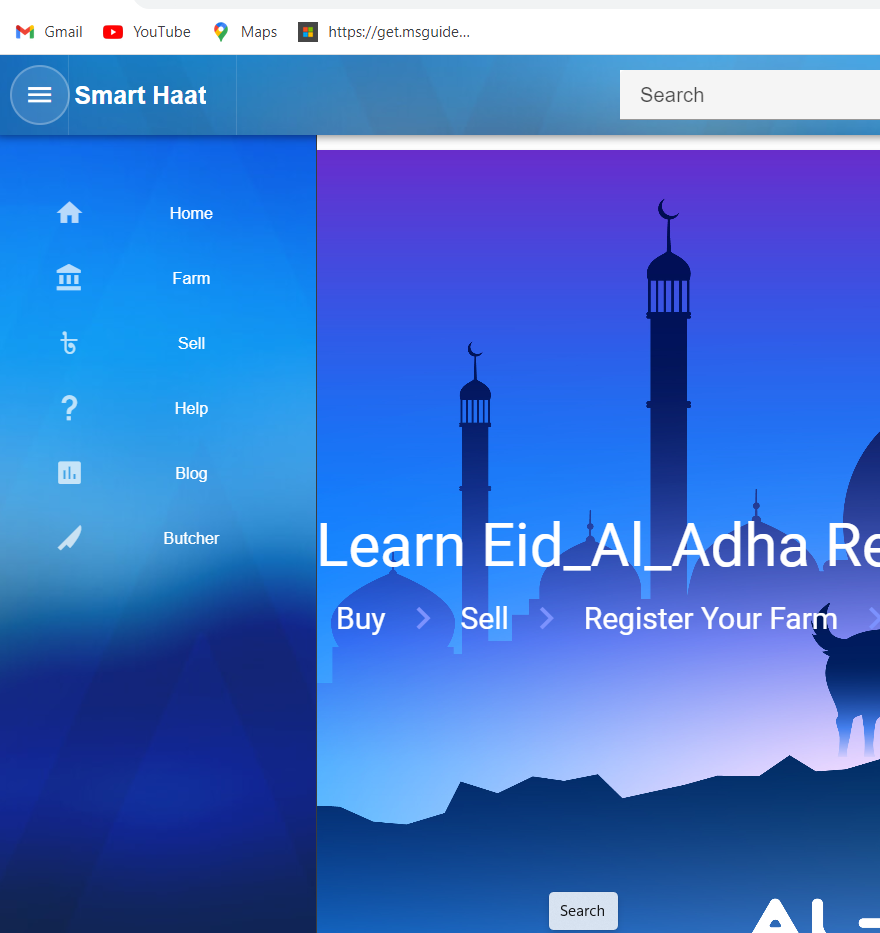
\includegraphics[keepaspectratio, width=10cm]{one.png}
\caption{Navigation drawer}
\label{drawer}
\end{figure}
A new theme setting is also added. Now a days themes are one of the most desired feature of a modern websites. And \emph{Toggle theme} button does the job here.
\begin{figure}[H]
\centering
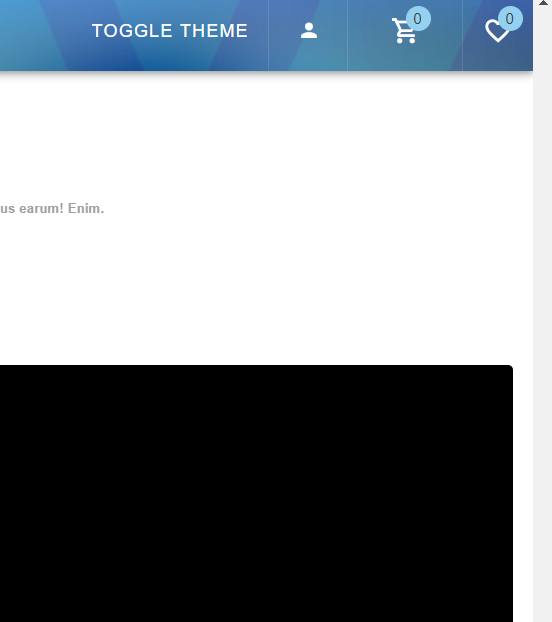
\includegraphics[keepaspectratio, width=10cm]{two.png}
\caption{Toggle theme}
\label{theme}
\end{figure}
The cart system is an improtant feature of an online selling websites. Thus the cart system is added here for customers. Here the user have to click the \emph{add to cart} button positioned beside every item. Finally in the \emph{my cart} page user can see the items added to be bought.
\begin{figure}[H]
\centering
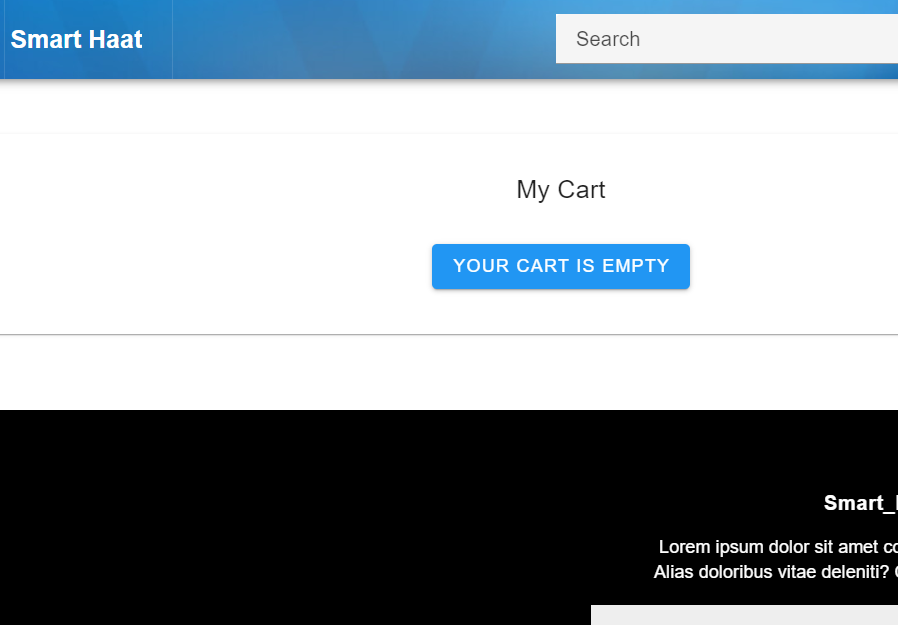
\includegraphics[keepaspectratio, width=10cm]{three.png}
\caption{Toggle theme}
\label{cart}
\end{figure}
Some more features of the home page have also been activated such as slide ranger, through which we can easily sort out the items easily.
\begin{figure}[H]
\centering
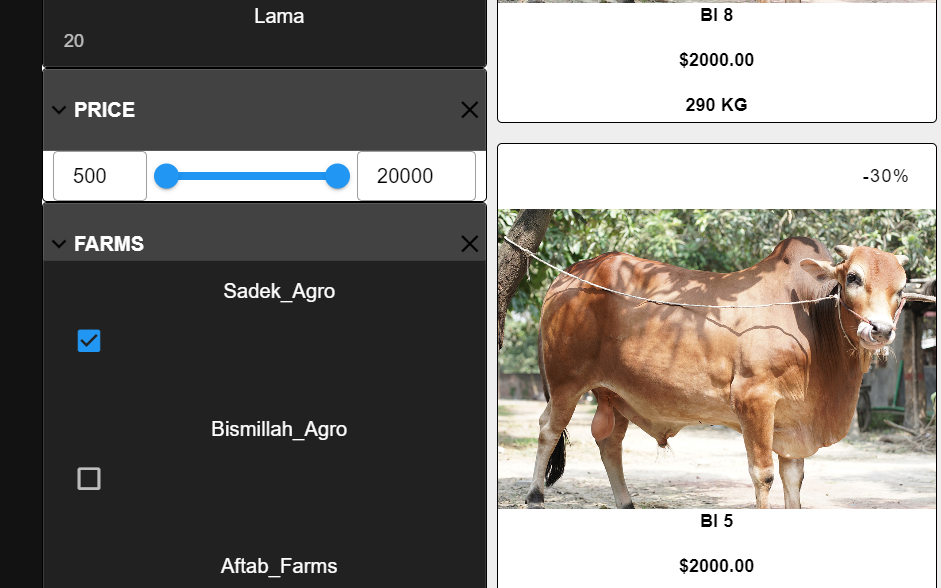
\includegraphics[keepaspectratio, width=10cm]{four.png}
\caption{Slide-ranger}
\label{slideranger}
\end{figure}
\section*{Development Platfroms}
The frameworks and language platforms we used --
\begin{itemize}
	\item HTML
	\item CSS
	\item JAVASCRIPT
	\item VUE
\end{itemize}

\section*{Conclusion}
This week we improved our home page with it's funtionalities and features. New cart system was developed. The login and signup page was made functional. Dark themes with other options were added. Due to some difficulties the database could not be added successfully and thats why the actual functions are not available.
\end{document}
